\documentclass[screen]{beamer}
\usepackage[T1]{fontenc}
\usepackage[latin1]{inputenc}

% Graphics
\RequirePackage{graphicx}
\RequirePackage{pdfpages}
\RequirePackage{wrapfig}
\RequirePackage{subfig}
\RequirePackage{caption}
\RequirePackage{tikz}
\RequirePackage{pgf}
\RequirePackage{pgfplots}
\usetikzlibrary{arrows,shapes,positioning,plotmarks}

% Color
\RequirePackage{xcolor}
\definecolor{red}{HTML}{990000}
\definecolor{green}{HTML}{336633}
\definecolor{black}{HTML}{000000}
\definecolor{lightgray}{HTML}{CCCCCC}
\definecolor{gray}{HTML}{999999}
\definecolor{darkgray}{HTML}{666666}

\usepackage{setspace}

% Bruk NTNU-temaet for beamer (her i bokmålvariant), alternativer er
% ntnunynorsk og ntnuenglish.
\usetheme{ntnuenglish}

\setbeamertemplate{footline}[ntnu theme nologo]
 
% Angi tittelen, vi gir også en kortere variant som brukes nederst på
% hver slide:
\title[Adaptive Aggregation of Recommender Systems]%
{Adaptive Aggregation of\\Recommender Systems}

% Angir foredragsholder, også en (valgfri) kortversjon i
% hakeparanteser først som kommer nederst på hver slide:
\author{Olav Bj{\o}rk{\o}y}

% Institusjon. Bruk gjerne disse slik det passer best med det du vil
% ha.  Valgfri kortversjon her også
\institute[NTNU]{Department of Computer and Information Science}

% Datoen blir også trykket på forsida. 
\date{October 3rd, 2011}
%\date{} % Bruk denne hvis du ikke vil ha noe dato på forsida.

% Fra her av begynner selve dokumentet
\begin{document}

% Siden NTNU-malen har en annen bakgrunn på forsida, må dette gjøres
% i en egen kommando, ikke på vanlig beamer-måte:
\ntnutitlepage
%\titlepage

% Her begynner første slide/frame, (nummer to etter forsida). 

\begin{frame}
  \frametitle{Terminology}
  \begin{tabular*}{1\textwidth}{ l l }
    \hline
    $u$ & user \\
    \hline
    $i$ & item (article, website, movie, product...)\\
    \hline
    $r$ & rating, relevance, utility (domain specific)\\
    \hline
    $m$ & a method for predicting ratings.\\
    \hline
    $p(m,u,i)$ & predicted rating of a method for $(u,i)$.\\
    \hline
  \end{tabular*}
\end{frame}

\begin{frame}
  \frametitle{2006: The Netflix Challenge}
    \begin{itemize}
      \item USD 1MM prize for a 10\% accuracy improvement.\\
      \item Breakthrough: Combining methods from many teams.\\
      \item Team BellKor finally achieved a 10.06\% improvement by combining \textbf{107} different recommender algorithms.
    \end{itemize}
\end{frame}

\begin{frame}
  \frametitle{Today: Web Search}
    \begin{block}{Google}
      "Today we use more than 200 signals, including PageRank, to order websites, and we update these algorithms on a weekly basis."
      \color{gray}{(\url{google.com/corporate/tech.html})}
    \end{block}
    \begin{block}{Bing}
      "We use over 1,000 different signals and features in our ranking algorithm."
      \color{gray}{(\url{bing.com/community/site_blogs/b/search/archive/2011/02/01/thoughts-on-search-quality.aspx})}
    \end{block}
\end{frame}

\begin{frame}
  \frametitle{Why multiple algorithms?}
  \begin{itemize}
    \item Use more data.
    \item Capture more predictive aspects.
    \item Disjoint predictors.
  \end{itemize}
  
  \begin{block}{Bell, R., Koren, Y., and Volinsky, C. (2007) (Netflix)}
    "Quite frequently we have found that the more accurate predictors are less useful within the full blend."
  \end{block}
\end{frame}

\begin{frame}
  \frametitle{The Problem: Latent Subjectivity}
  \begin{eqnarray}
    \hat{r}_{u,i} = \sum_{m \in M} w_{m} \times p_{r}(m,u,i)
  \end{eqnarray}
  \begin{itemize}
    \item Generalized optimal weights.
    \item Treats all users and items the same.
    \item Varying accuracy across users.
    \item Varying accuracy across items.
    \item A case of misplaced subjectivity.
  \end{itemize}
\end{frame}

\begin{frame}
  \frametitle{The Problem: Latent Subjectivity}
  \huge
  \linespread{2}{
    Systems that insist on being adaptive in a certain way
    are not really adaptive at all.  
  }
\end{frame}

\begin{frame}
  \frametitle{Adaptive Recommenders}
  \begin{eqnarray}
    \hat{r}_{u,i} = \sum_{m \in M} p_{w}(m,u,i) \times p_{r}(m,u,i)
  \end{eqnarray}
  \begin{itemize}
    \item $p_r$: predicted rating from method $m$ for $(u,i)$.
    \item $p_w$: predicted optimal weight for method $m$ for $(u,i)$.
    \item We can use standard recommenders for both $p_r$ and $p_w$.
  \end{itemize}
\end{frame}

\begin{frame}
  \begin{figure}
  \center
  \def\layersep{1.8cm}
  \begin{tikzpicture}[shorten >=1pt,->,draw=black, node distance=\layersep]

    \tikzstyle{every pin edge}=[<-,shorten <=2pt]
    \tikzstyle{node}=[circle,fill=black!25,minimum size=20pt,inner sep=0pt]
    \tikzstyle{input node}=[node, fill=green!25];
    \tikzstyle{output node}=[node, fill=red!25];
    \tikzstyle{hidden node}=[node, fill=blue!25];
    \tikzstyle{annot} = [text width=10em, text centered]
    \tikzstyle{txt}=[node,fill=white];
    
    \node[txt] (UI) at (0,-2) {$(u,i)$};  

    \node[input node] (I-1) at (\layersep,-1) {$m_1$};
    \node[txt]        (I-D) at (\layersep,-2) {$\vdots$};
    \node[input node] (I-N) at (\layersep,-3) {$m_n$};
    
    \node[txt] (P-1) at (\layersep*2, -1) {$p_1$};
    \node[txt] (P-D) at (\layersep*2, -2) {$\vdots$};
    \node[txt] (P-N) at (\layersep*2, -3) {$p_n$};

    \node[hidden node] (H-1) at (\layersep*3, -1) {$a_1$};    
    \node[txt]         (H-D) at (\layersep*3, -2) {$\vdots$};    
    \node[hidden node] (H-N) at (\layersep*3, -3) {$a_n$};    

    \node[txt] (R-1) at (\layersep*4, -1) {$(p_1,w_1)$};
    \node[txt] (R-D) at (\layersep*4, -2) {$\vdots$};
    \node[txt] (R-N) at (\layersep*4, -3) {$(p_n,w_n)$};
    
    % hidden helper node
    \node[txt] (HH)  at (\layersep*5,-1) {};

    % Draw the output layer node
    \node[output node,pin={[pin edge={->}]right:$\hat{r}$}] at (\layersep*5,-2) (O) {$\Sigma$};
    
    \path (UI) edge (I-1);
    \path (UI) edge (I-N);

    \path (I-1) edge (P-1);
    \path (I-N) edge (P-N);

    \path (P-1) edge (H-1);
    \path (P-N) edge (H-N);

    \path (H-1) edge (R-1);
    \path (H-N) edge (R-N);

    \path (R-1) edge (O);
    \path (R-N) edge (O);

    % Annotate the layers
    \node[annot,above of=I-1, node distance=1cm] {\emph{prediction}};
    \node[annot,above of=H-1, node distance=1cm] {\emph{adaption}};
    \node[annot,above of=HH,  node distance=1cm] {\emph{aggregation}};
  \end{tikzpicture}

  \vspace{1em}
  \caption[The Layers of Recommenders]{
    Layers of recommenders. 
  }
  \label{fig:adaptiveusermodeling}
\end{figure}

\end{frame}

\begin{frame}
  \frametitle{Training phase}
  
  \begin{itemize}
    \item Split into two sets using bootstrap aggregation: $(d_m,d_e)$.
    \item Use $d_m$ to train the basic recommenders.
    \item Create an error matrix using the basic recommenders and $d_e$. 
    \item The error matrix values are predicted errors for $(u,i,m)$.
    \item Train adaptive recommenders on the error matrix.
  \end{itemize}
  
  \begin{eqnarray}
    \forall (u,i,r) \in (d_e - d_m): E(m)_{u,i} = |r - p(m,u,i)|
  \end{eqnarray}
\end{frame}

\begin{frame}
  \begin{equation*}
     R_{u,i} =
     \begin{pmatrix}
      r_{1,1} & r_{1,2} & \cdots & r_{1,i} \\
      r_{2,1} & r_{2,2} & \cdots & r_{2,i} \\
      \vdots  & \vdots  & \ddots & \vdots  \\
      r_{u,1} & r_{u,2} & \cdots & r_{u,i}
     \end{pmatrix}
    \end{equation*}

  \vspace{1em}
  
    \begin{equation*}
     E_{u,i} =
     \begin{pmatrix}
        e_{1,1} & e_{1,2} & \cdots & e_{1,i} \\
        e_{2,1} & e_{2,2} & \cdots & e_{2,i} \\
        \vdots  & \vdots  & \ddots & \vdots  \\
        e_{u,1} & e_{u,2} & \cdots & e_{u,i}
     \end{pmatrix}
    \end{equation*}
    
    \vspace{1em}
    \begin{center}
      Train $p_r$ with $R$ and $p_w$ with $E$.
    \end{center}
\end{frame}

\begin{frame}
  \frametitle{Prediction phase}
  
  \begin{itemize}
    \item Calculate each prediction $\hat{r}_{(u,i,m)}$.
    \item Calculate each predicted error $\hat{e}_{(u,i,m)}$.
    \item The adaptive weights are the inverses of the normalized error.
    \item Sum the weighted predictions to get the final $\hat{r}$.
  \end{itemize}  
\end{frame}

\begin{frame}
  \begin{equation}
    \label{eq:adaptive}
    \hat{r}_{u,i} = \sum_{(m_{e}, m_{r}) \in M} (1 - 
    \frac{
      p(m_{e},u,i)
    }{
      error(u,i)
    }) \times p(m_{r},u,i)
  \end{equation}
  \vspace{2em}
  \begin{equation}
    error(u,i) = \sum_{m_e \in M} p(m_e,u,i)     
  \end{equation}
\end{frame}

\begin{frame}
  \frametitle{Results}
  \begin{itemize}
    \item Calculate RMSE values for basic recommenders, simple aggregations and adaptive aggregation.
    \item Used the Movielens movie rating dataset (see paper for more details).
    \vspace{2em}
    \begin{equation}
      \mathrm{RMSE}(\hat{R},R)
      = \sqrt{\frac{
          \sum_{i=1}^{n} (\hat{R}_i - R_i)^2
        }{
          n
        }}
    \end{equation}
  \end{itemize}
\end{frame}

\begin{frame}
  \begin{table}
  
  \centering
  \tiny
  (a) RMSE values for the five disjoint subsets:

  \vspace{0.4em}

  \begin{tabular*}{0.9\textwidth}{ l l l l l l l }
    \hline
    { } & method & $d_1$ & $d_2$ & $d_3$ & $d_4$ & $d_5$ \\ 
    \hline
    S & svd1          & 1.2389	  & 1.1260	  & 1.1327	  & 1.1045	  & 1.1184	 \\
    S & svd2          & 1.2630	  & 1.1416    & 1.1260	  & 1.1458	  & 1.1260	 \\
    S & svd3          & 1.0061	  & 0.9825	  & 0.9830	  & 0.9815	  & 0.9797	 \\
    S & svd4          & 1.0040	  & 0.9830	  & 0.9849	  & 0.9850	  & 0.9798	 \\
    S & slope\_one    & 1.1919	  & 1.0540	  & 1.0476	  & 1.0454	  & 1.0393   \\
    S & item\_avg     & 1.0713	  & 0.9692	  & 0.9662	  & 0.9683	  & 0.9725	 \\
    S & baseline       & 1.0698	  & 0.9557	  & 0.9527	  & 0.9415	  & 0.9492	 \\
    S & cosine   	    & 1.1101	  & 0.9463	  & 0.9412	  & 0.9413	  & 0.9382	 \\
    S & knn       	  & 1.4850	  & 1.1435	  & 1.1872    & 1.2156	  & 1.2022	 \\
    \hline                                                                    
    A & median    	  & 0.9869	  & 0.8886	  & 0.8857    & 0.8857	  & 0.8855	 \\
    A & average    	  & 0.9900	  & 0.8536	  & 0.8525	  & 0.8525	  & 0.8519	 \\
    A & adaptive       & \textbf{0.9324}	  & \textbf{0.8015}	  & \textbf{0.7993}  & \textbf{0.8238} & \textbf{0.8192} \\
    \hline
  \end{tabular*}

  \vspace{1em}
  
  (b) Statistics for the methods:

  \vspace{0.4em}

  \begin{tabular*}{0.9\textwidth}{ l p{1.8cm} l l l l l }
    \hline
    { } & method & min & max & mean & $\sigma$ & $\Delta$ \\
    \hline
    S & knn       	  & 1.1435	& 1.4850	& 1.2467	& 0.3487 & - \\
    S & svd2          & 1.1260	& 1.2630	& 1.1605	& 0.2277 & 6.9\% \\
    S & svd1          & 1.1045	& 1.2389	& 1.1441	& 0.2197 & 1.4\% \\
    S & slope\_one    & 1.0393	& 1.1919	& 1.0756	& 0.2415 & 5.9\% \\
    S & item\_avg     & 0.9662	& 1.0713	& 0.9895	& 0.2023 & 8.0\% \\
    S & svd4          & 0.9798	& 1.0040	& 0.9873	& \textbf{0.0924} & 2.2\% \\
    S & svd3          & 0.9797	& 1.0061	& 0.9865	& 0.0991 & 0.1\% \\
    S & cosine   	    & 0.9382	& 1.1101	& 0.9754	& 0.2595 & 1.1\% \\
    S & baseline       & 0.9415	& 1.0698	& 0.9738	& 0.2196 & 1.6\% \\
    \hline            
    A & median    	  & 0.8855	& 0.9865	& 0.9065	& 0.2005 & 6.9\% \\
    A & average    	  & 0.8519	& 0.9900	& 0.8801	& 0.2344 & 2.9\% \\
    A & adaptive       & \textbf{0.7993}	& \textbf{0.9324}	& \textbf{0.8352}	& 0.2225 & 5.1\% \\
    \hline
  \end{tabular*}
  \label{table:results:e1}
\end{table}
\end{frame}

\begin{frame}
  \begin{figure}[t]
\center

\pgfplotsset{width=\textwidth,height=8cm}
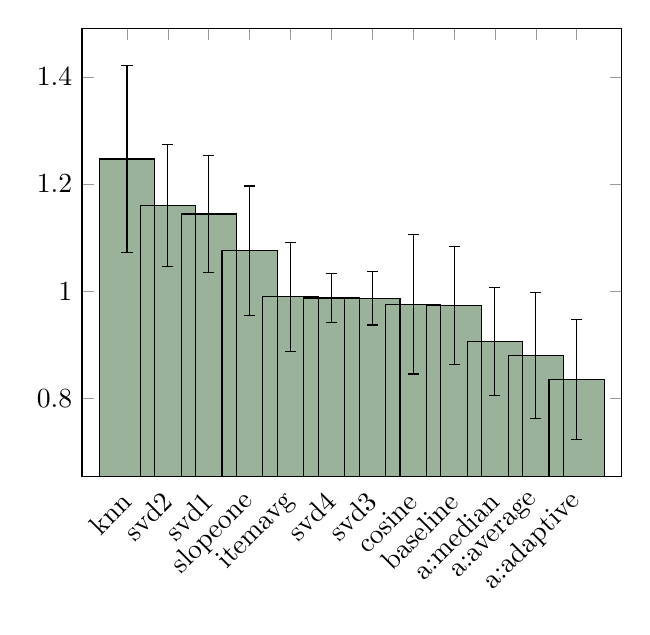
\begin{tikzpicture}

\begin{axis}[
      symbolic x coords={
        knn,svd2,svd1,slopeone,itemavg,svd4,svd3,cosine,baseline,a:median,a:average,a:adaptive},
      xtick=data,
      x tick label style={rotate=45,anchor=east,yshift=-0.5em,xshift=-0.2em},
      bar width=20pt
    ]

    \addplot [ybar,fill=green!50,error bars/.cd,y dir=both,y explicit] coordinates {
      (knn, 1.2467) +- (0,0.17435) 
      (svd2, 1.1605) +- (0,0.11385)
      (svd1, 1.1441) +- (0,0.10985)
      (slopeone, 1.0756) +- (0,0.12075)
      (itemavg, 0.9895) +- (0,0.10115)
      (svd4, 0.9873) +- (0,0.0462)
      (svd3, 0.9865) +- (0,0.04955)
      (cosine, 0.9754) +- (0,0.12975)
      (baseline, 0.9738) +- (0,0.1098)
    %};
    %\addplot [ybar,fill=blue!50] coordinates {
      (a:median, 0.9065) +- (0,0.10025)
      (a:average, 0.8801) +- (0,0.1172)
      (a:adaptive, 0.8352) +- (0,0.11125)
    };
\end{axis}

\end{tikzpicture}
\caption[Average RMSE Plot]{
  Average RMSE plot: This plot shows the average RMSE for each method, and each aggregation method (denoted "a:").
  The actual numbers are given in Table \ref{table:results:e1}.
  The error bars indicate the standard deviation of each method.
  Note the scale on the y-axis --- the errors are not as pronounced as they might seem. 
  See also Figure \ref{plot:datasets}.
}
\label{plot:rmse}
\end{figure}




\end{frame}

\begin{frame}
  \begin{figure}
\center

\pgfplotsset{width=\textwidth,height=8cm}
\pgfplotsset{every axis/.append style={
thick,
tick style={semithick}}}

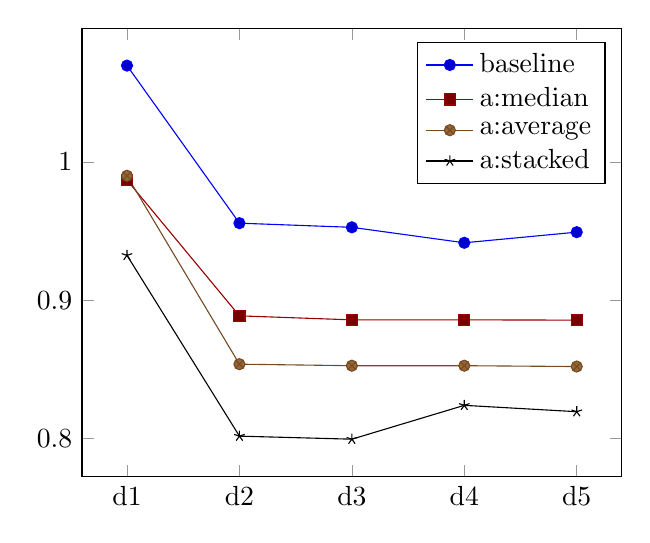
\begin{tikzpicture}

\begin{axis}[
  stack plots=false,
  enlarge x limits=true,
  symbolic x coords={d1,d2,d3,d4,d5},
  xtick=data,
  legend style={
    cells={anchor=west},
    legend pos=north east,
  }
]

\addplot coordinates {
(d1, 1.0698)
(d2, 0.9557)
(d3, 0.9527)
(d4, 0.9415)
(d5, 0.9492)
};
\addlegendentry{baseline}


\addplot coordinates {
(d1, 0.9869)
(d2, 0.8886)
(d3, 0.8857)
(d4, 0.8857)
(d5, 0.8855)
};
\addlegendentry{a:median}
 
\addplot coordinates {
(d1, 0.9900)
(d2, 0.8536)
(d3, 0.8525)
(d4, 0.8525)
(d5, 0.8519)
};
\addlegendentry{a:average}
 
\addplot coordinates {
(d1, 0.9324)
(d2, 0.8015)
(d3, 0.7993)
(d4, 0.8238)
(d5, 0.8192)
};
\addlegendentry{a:stacked}

\end{axis}
\end{tikzpicture}

\caption[RMSE Variations]{
  RMSE Variations: This plot shows that, while the standard deviation of each method may be high,
  this has more to do with the selected dataset than with their performance in comparison with each other.
  The performance of each of the aggregate methods, as well as the baseline standard method,
  follow similar performance paths across the disjoint datasets.
}
\label{plot:datasets}
\end{figure}





\end{frame}

\begin{frame}
  \frametitle{Limitations}
  \begin{itemize}
    \item Lots of added complexity for fairly unknown improvement.
    \item Only tested on a few datasets, no real world situations.
    \item Only compared to simple aggregation methods.
    \item Neither the aggregators nor the basic recommenders were
      heavily optimized to the domain of the dataset.
  \end{itemize}
\end{frame}

\begin{frame}
  \frametitle{Adaptive Recommenders}
  \begin{itemize}
    \item Combine disjoint algorithms
    \item Weight recommenders by predicted accuracy.
    \item Accuracy predictions are contextually dependent on $(u,i,m)$.
    \item \emph{Any} applicable recommender becomes a worthy addition.
    \item See paper for references and more results.
  \end{itemize}
\end{frame}

\end{document}